% Chapter 2

\chapter{Project management} % Main chapter title

\label{Chapter2} % For referencing the chapter elsewhere, use \ref{Chapter1} 

\lhead{Chapter 2. \emph{Project management}} % This is for the header on each page - perhaps a shortened title

%----------------------------------------------------------------------------------------
In this chapter we want to present how our group organized and managed this project. Group members are:
\begin{itemize}
\item Oksana Hagen
\item Natalia Shepeleva
\item Emre Ozan Alkan
\item Klemen Istenič
\end{itemize}
As we all had a bit of experiences in software design, we knew how important a proper plan and research before the actual implementation is. Unfortunately, we were also aware that no matter how good the plan is, we will be forced to adjust it during the implementation. Either because of the things we overlooked while planning or because some assumptions we made were wrong. We decided to follow the \textit{iterative and incremental development model}, which enabled us to adjust our plans after each of the implementation iterations. A schematic representation of the iterative and incremental development model can be seen on figure \ref{fig:Iterative_development_model_V2}.
\begin{figure}[h]
\centering
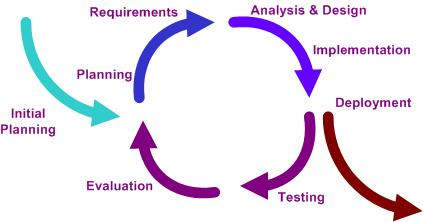
\includegraphics[height=4cm]{../pictures/Iterative_development_model_V2}
\caption{An iterative development model (image taken from \cite{wiki1})}
\label{fig:Iterative_development_model_V2}
\end{figure}

\section{Basic building blocks}
\label{Building blocks}
On our first meeting we decided to split the project into four main parts to be able to fully manage the whole project at all times. This parts are:
\begin{itemize}
\item User interface
\item Database and data structure
\item Map representation
\item Path algorithms
\end{itemize}

\subsection{UI - User Interface}
Part of the application that is responsible for user interaction with the application. Main goal is to make the interface as user-friendly as possible. In the beginning we made a rough sketch of how the interface should look (figure \ref{fig:sketch}), which has, as expected, changed during the process of later design and implementation. The UI is presented more in details in chapter [UI USER MAUNAL].
\begin{figure}[h]
\centering
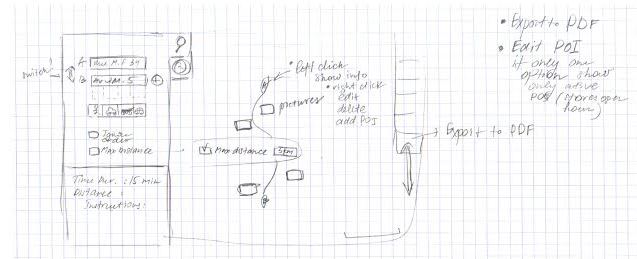
\includegraphics[width=0.6\linewidth]{../pictures/sketch.jpg}
\caption{Inital sketch of UI}
\label{fig:sketch}
\end{figure}
\subsection{Database and data structure}
Our database consists of two parts. The static part, having the information about the roads in Le Creusot (described in []) and the dynamic part with the information about the points of interest (POI). In chapter[] we address the facts we took into account while considering different database options and data structures.
\subsection{Map representation}
We separated map representation from other parts of user interface, because we think it is the most important of UI, so we will give special attention to it.
\subsection{Path algorithms}
In the different algorithms we adopted and developed, we do all the searching for paths, calculating distance and travel times and optimize the search results as much as possible. Our main goal is to make the algorithms work as  quickly as possible, taking into account all the restrictions road networks has (one way streets, foot ways etc.). We also want to make the algorithms as reusable as possible, to reduce the redundancy in development and minimize the possibilities of errors.


\section{Meetings and Project Progress}

Development stages can be divided in three parts. First stage included analyzing the problem, extracting project requirements and devising a plan for the implementation. Second part included extracting the application structure, collecting most appropriate tools for the implementation and setting up the environment. The last part is the implementation itself starting from building the basic blocks, simple prototype application and then gradually adding functionalities and features, along wise with documenting the software. All the stages were supported with meetings according to time constraints and project progress speed.

\subsection{Analyzing the problem}
Fist meetings were devoted to the analyzing the provided requirements and inventing all possible useful features. Besides the general idea of user interface was developed according to all the needed functionality of the project. The scope of the project was defined and future work planned.

\subsection{Pre-implementation stage}
In the later meetings we were considering architecture challenges and possible solutions, able to provide the need functionality for the application. We were focusing on extracting the most appropriate tools and libraries to ease the development process as well as getting the idea . After it was done the same development environment was set up on all the computers. At this point it was clear how the implementation will differ in Matlab and C++ and the team got slitted between Matlab and C++ development.

\subsection{Implementation}
All next meetings were devoted to the coding the application and solving particular issues. At this stage separate basic blocks (ui, map-rendering, database, algorithms) were developed and then merged in one working application prototype, which only consisted of two-point path search. When it was clear that all the framework decisions were reasonable, further development was done.

\section{Software used for project management}
At first and second stage Dropbox was used to share latest meeting reports, schematics, useful papers and links. On the last stage the need of tool for simultaneous development became obvious. For that purpose, we chose GitHub repository hosting service. Besides, it was extremely useful for tracking issues and bugs. At very last meetings we used Skype conferences, since all the project team members were in different places.
